\section{Konečný stavový automat}
\noindent Existuje množstvo spôsobov ako modelovať správanie sytémov. Jedným z 
najstarších a najznámejších je modelovanie pomocou konečného stavového automatu.
Vďaka takejto abtrakcii môžeme o problémoch rozmýšľať ako o stavoch, ktoré nastali v určitom čase a charakterizujú to ako sa systém má správať. Táto technika však nieje limitovaná len na modelovanie softvérových systémov. Využíva sa aj v iných oblastiach ako napríklad vo fyzike a biológii \cite{WaybackMachine2014}. \par 
Konečný stavový automat je je výpočtový model, ktorý sa používa na simuláciu sekvenčnej logiky. Poznáme dva typy konečných stavových strojov: deterministický konečný automat (DKA)  a nedeterministický stavový automat (NKA) \cite{FiniteStateMachines}. 

\subsection{Deterministický konečný automat}
\noindent Deterministický konečný automat $\mathcal{M}$ je definovaný päticou ($\Sigma$ ,$\mathcal{Q}$ , $q_0$, $\mathcal{F}$, $\delta$) kde
\begin{itemize}
    \item $\Sigma$ je neprázdna a konečná množina vstupná abeceda $\mathcal{M}$
    \item $\mathcal{Q}$ je konečná množina stavov $\mathcal{M}$
    \item $q_0$ je počiatočný stav $\mathcal{M}$
    \item $\mathcal{F}$ $\subseteq$ $\mathcal{Q}$ je množina konečných stavov $\mathcal{M}$
    \item $\delta$ je prechodová funkcia  \begin{math}\delta : Q \times \Sigma \Rightarrow Q\end{math}
\end{itemize}

Automat musí definovať presne jednu prechodovú funkciu pre každý symbol v $\Sigma$ pre každý stav v $\mathcal{Q}$. DKA môže byť reprenzentovaný aj pomocou diagramu ktorý vidíme na obrázku \ref{dfa1}.

\begin{figure}[h]
    \centering
    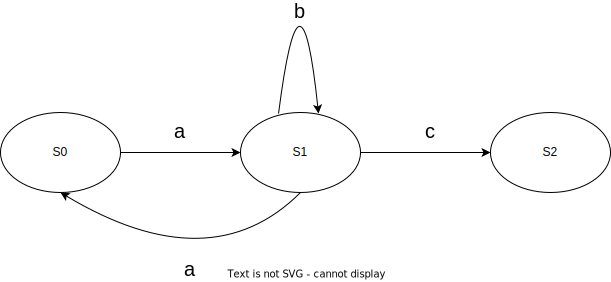
\includegraphics[width=0.75\textwidth]{img/dfa.png}
    \caption{Príklad deterministického konečného stavového automatu}
    \label{dfa1}
\end{figure}

